\chapter{Benchmarks and Discussion}

We will present a number of benchmarks designed to compare and
quantify the differences in performance of the parallelization models
that we have implemented.

Since the execution time is only dependent on the total amount of work
that a network performs and not how the processes in the network are
connected, all of our benchmarks will use a ring-shaped
(\cref{fig:benchnetwork}) network with the participating processes
performing varying amounts of work.

We conjecture that the scalability of our implementation will depend
strongly on the nature of the workload performed by the SME-networks
benchmarked. We will therefore benchmark both light and heavy

As our previously presented hypotheses states, we expect our
benchmarks to show that the effects of syncing becomes more pronounced
as we decrease the amount of work performed by our processes while it,
on the other hand, will become amortized as the amount of work
performed by each process increases.

\begin{figure}
\centering
\includegraphics{figures/ring}
\caption[SME network used for benchmarking]{Illustration showing the
  layout of the network used for benchmarking. The blue circles
  represents processes and the arrows represents busses}
\label{fig:benchnetwork}
\end{figure}


\section{Testing methodology}
All of the time measurements shown were performed inside the SME
framework itself using the C++11 \texttt{<chrono>} functions, and
measures only the actual execution time of the network. It therefore
does not include the constant time required to generate the
benchmarked networks. Two different hardware platforms has been used
for performing the benchmarks: One AMD and one Intel platform.

The Intel machine has the following specs
\begin{itemize}
\item CPU: 1x Intel Xeon E3-1245 V2 @ 3.40GHz, 4 cores (8 threads)
\item RAM: 32GB
\item OS: Linux
\end{itemize}

and the AMD machines used are part of the eScience cluster at NBI and
boasts the following specs:
\begin{itemize}
  \item CPU: 2x AMD Opteron 6272 @ 2.1GHz, 16 cores
  \item RAM: 128GB
\end{itemize}

Since the instruction set used by the two CPU's support incompatible
optimizations, code generated for one of the CPU's will not run
unmodified on the other. Therefore, code executed on the AMD CPU were
compiled with the GCC flags \texttt{-mtune=barcelona
  -march=barcelona}, while code executed on the Intel CPU were
compiled with \texttt{-march=native} on a Core i7 machine. GCC 4.9 was
used in both cases. Furthermore, due to incompatible versions of
\texttt{libstdc++} on the test machines, all benchmarks has been
performed using statically linked binaries.

All of the benchmarks has been executed 5 times and the graphs are
based on the averages of these. Error bars showing the minimum and
maximum deviation from the average has been added to all graphs,
however, in some cases the deviations between benchmark runs were too small
for the error bars to be visible.
We have tried to size the workloads such that the running times are
kept within reasonable bounds \fxnote{elaborate}
We calculate our speedup using the formula


\begin{equation*}
S = \frac{T_{\text{old}}}{T_{\text{new}}}
\end{equation*}

where $S$ is the achieved speedup, $T_{\text{old}}$ is the original
(pre-improvement) speed and $T_{\text{new}}$ is the new
(post-improvement) speed \cite{hennessy2012computer}.

As a final note, when we talk about the workload of a cycle we refer
to the combined work of all processes in the network, not the work
performed by an individual process. As such, we define the workload of
the network as a function of both the work performed by the individual
processes and the number of processes participating in the
network. The raw benchmark data can be found in \cref{chap:benchdata}.

\section{Synchronization dominated}
In this section, we present a benchmark where the performance is
predominantly determined by the efficiency of the synchronization
mechanisms.

We perform this benchmark by creating a ring which does nothing other
than passing an integer value from process to process. Sine each
process only takes a few clock cycles to execute, we expect that this
benchmark will expose the overhead caused by synchronization.

The following source code used in the execution unit of the process
\begin{listing}
\begin{minted}{C++}
void step() {
  int val = in->read();
  out->write(++val);
}
\end{minted}

\caption{Source code for the execution unit of the processes
  participating in the network used for sync-dominated benchmarking}
\end{listing}

\begin{figure}
\centering
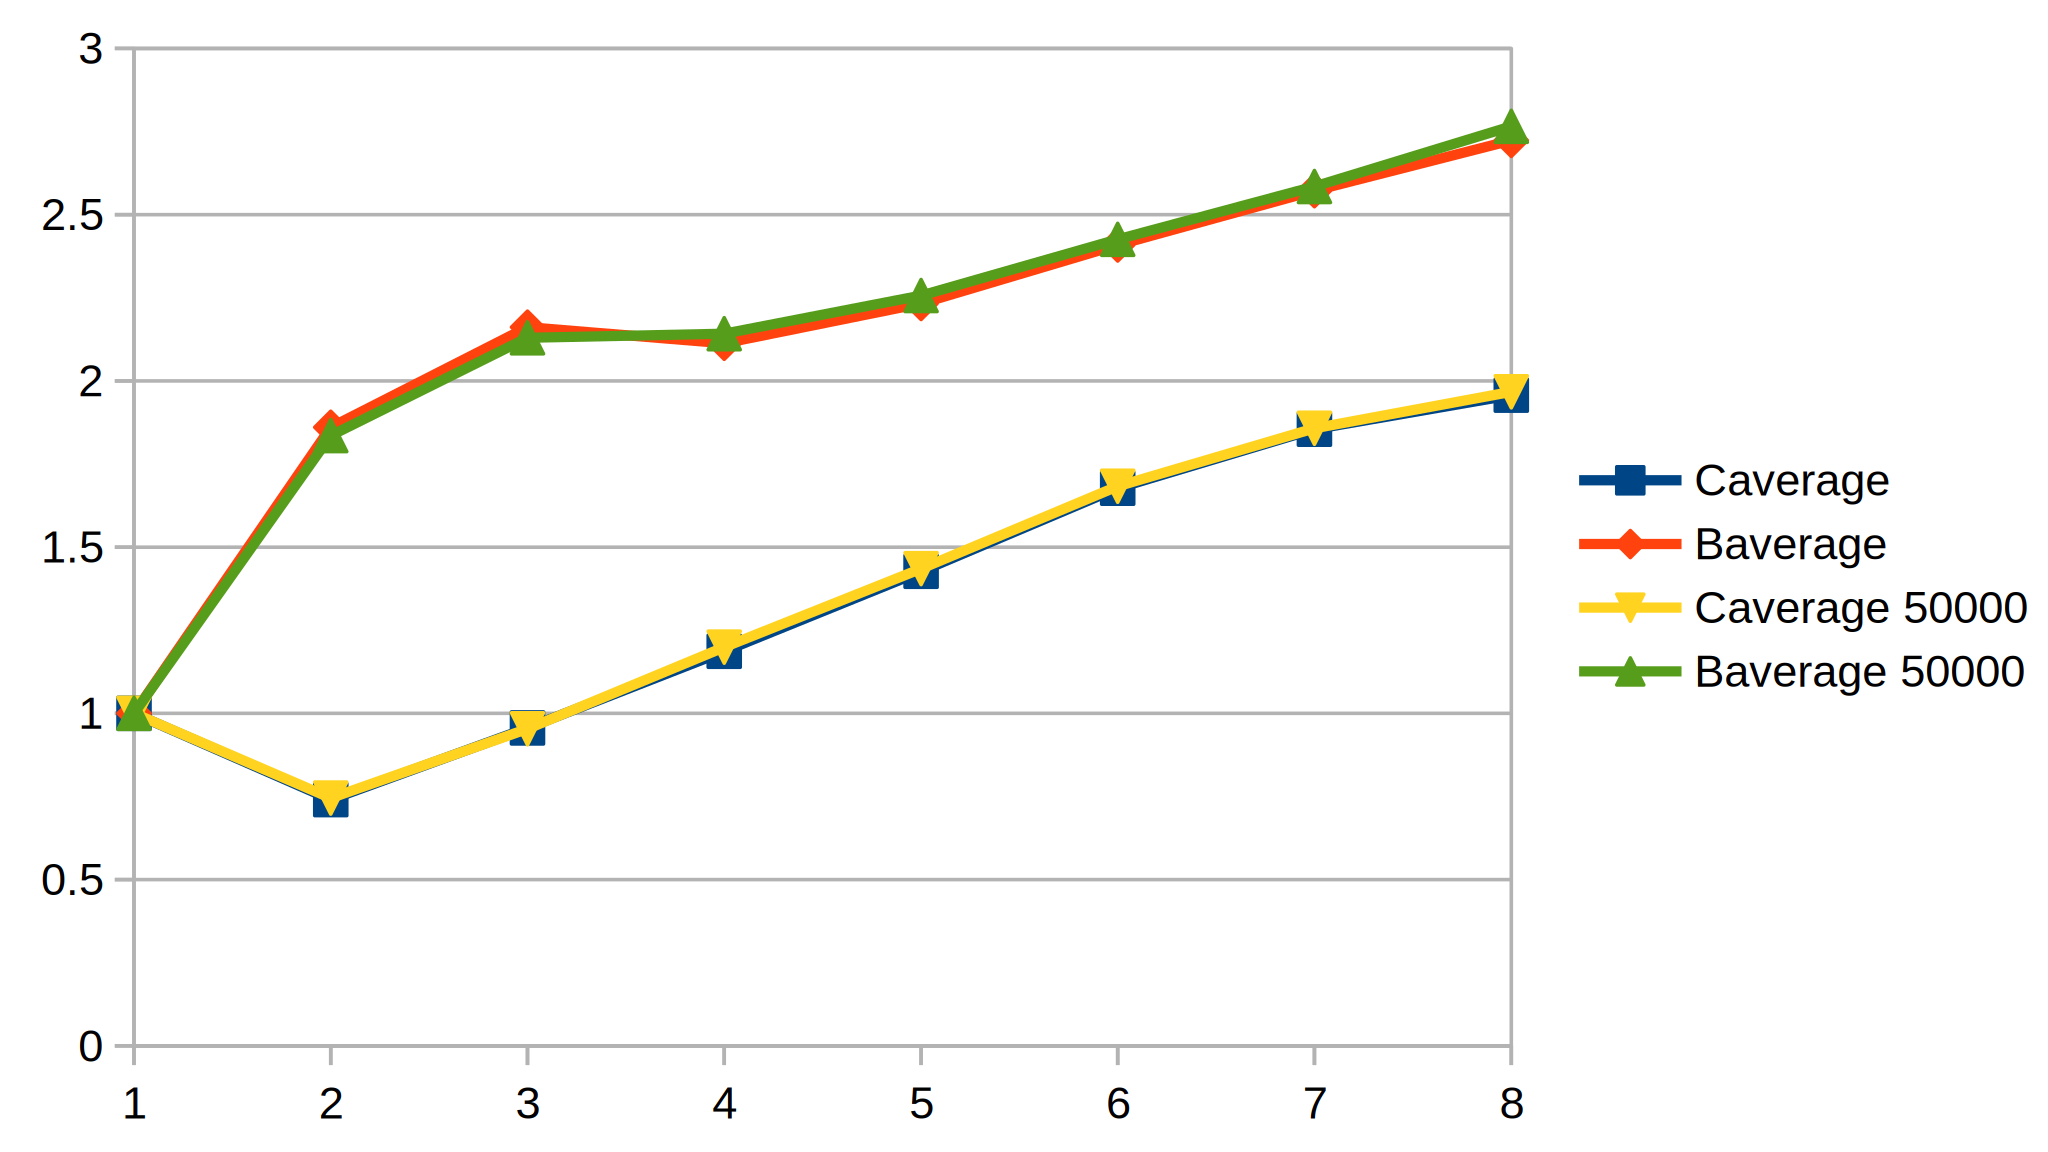
\includegraphics[width=\textwidth]{graphs/graphone}
\caption[Benchmark graph]{Graph showing the speedup of a SME network
  consisting of 20000 and 50000 processes respectively when executed
  for 50000 cycles on an Intel Xeon CPU}
\label{fig:intel-sync}
\end{figure}

\begin{figure}
\centering
\includegraphics[width=\textwidth]{graphs/amd-sync-20000}
\caption[Synchronization-dominated benchmark on AMD cluster]{Benchmark results for a network of 20000 processes running
for 100000 iterations on the AMD cluster}
\label{fig:amd-sync}
\end{figure}


\subsection{Discussion}
We can observe a number of things from the results that can bee seen
in \cref{fig:intel-sync}.  This benchmarks shows the performance of
two different networks, one with 20000 processes and one with 50000
processes. Both networks executed 100000 cycles.

When looking at the benchmark of the worker list model, one thing that
is clearly visible from this benchmark is the overhead produced by the
atomic increment that is required.. This model is doubly penalized
when running the benchmark since we, addition to then time required by
the atomic increment, which is performed before every process
execution, also need to wait for all of the threads to sync
up at the end of a cycle. What is slightly surprising, however, is the
actual performance that this method shows. It performs significantly
worse when going from one to two threads. The most likely explanation
for this result is CPU optimizations which make atomic updates of a
variable less costly when these updates only occures from one thread.

Our static orchestration model performs quite decently and produces
almost 2x speedup when going from 1 to 2 threads. When adding
additional threads, the speedup decreases, which is expected since the
time spent synchronizing is increased,

%\fxnote{which manifests as
%  dropping CPU-utilization. When running 4 threads, the CPU
%  utilization drops to 360\%, unfortunately, I probably wont have time
%  to measure or show this}

Common for both of the models, is that the size of the network
executed seems to have no impact on the relative speedups achieved.

Since the Xeon CPU that the benchmarks were performed on only have 4
cores with Hyper Threading, another interesting observation is that
Hyper Threading seems to give a significant additional speedup. One
hypothesis for explaining the cause of this is that branch-prediction
isn't very effective at predicting which functions we're going to call
in our SME network. A branch mis-prediction causes the CPU-pipeline to
be cleared, creating an optimal condition for Hyper Threading to make
use of the empty pipeline-stages\cite{fog2014microarchitecture} While
branch-predictors This hypothesis could be tested by running the
program through a profiler in order to measure the number of
mis-predictions occurring. At this time, these results are not
available.

\Cref{fig:amd-sync} show the results of the smallest version of the
benchmark running on the AMD cluster. The results are significantly
worse compared to the results of the Intel Xeon CPU, both in absolute
running times \fxnote{Is it OK to show the numbers?} and
speedup. Early possible explanations was that, due to the extremely
long running time of the benchmark, we were seeing the effects of the
process being moved between CPU-cores. However, the results remained
unchanged after pinning the threads to CPU-cores placed on the same
NUMA-unit. Thus, the only reasonable explanation explanation is that our
syncronization mechanisms is significantly less optimized on the AMD
CPU compared to the Intel CPU.

Another thing standing out from this benchmark is the huge variability
between the different benchmark runs as shown by the Y-axis error bars.

Due to these very poor initial benchmark results, we didn't attempt
benchmark the synchronization dominated network with different problem
sizes on the AMD-cpu.


\section{Cycle dominated}

\begin{figure}
\centering
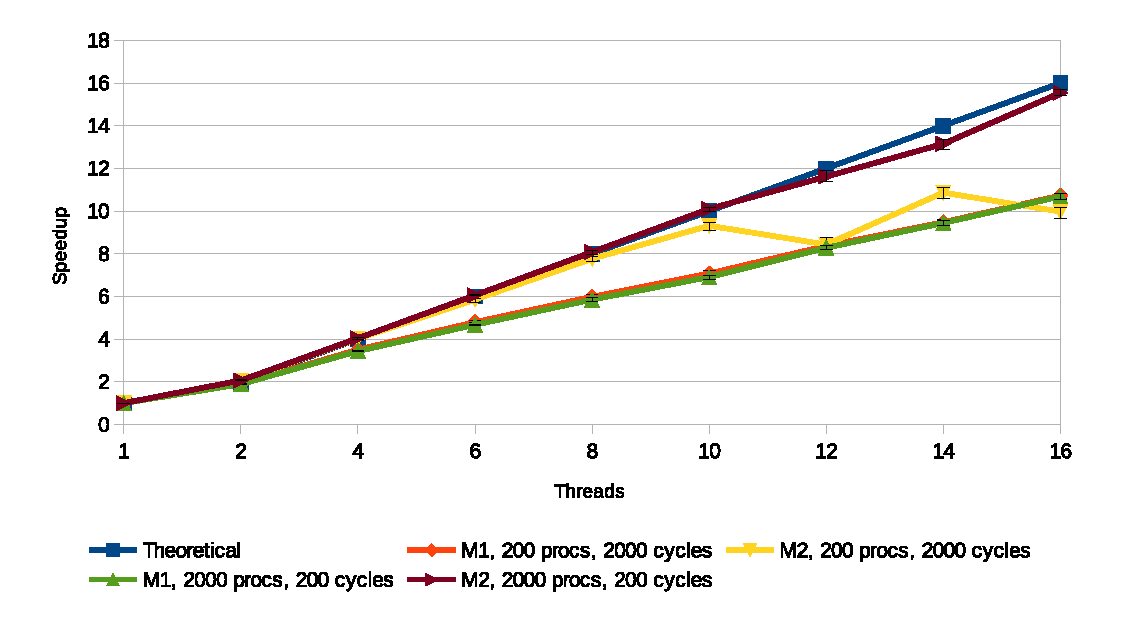
\includegraphics[width=\textwidth]{graphs/heavy-ring2}
\caption[Synchronization-dominated benchmark on AMD cluster]{Benchmark results for a network of 20000 processes running
for 100000 iterations on the AMD cluster}
\label{fig:heavy-ring}
\end{figure}


In this benchmark, the processes in the network performs a significant
amount work. We expect that this will, to some extent, amortize the
synchronization overhead inherent in the SME model. Combined with the
fact that the individual processes contain no shared state, we
conjecture that this benchmark will scale significantly better
than the previous synchronization dominated benchmark that we
performed.

The unit of work being performed by every process in every cycle is
simply to divide a \texttt{double} floating point number by 3, 10000
times. Since the busses in our SME-implementation only supports
transporting integer values nothing is being done with the value calculated,
but as long as our workload isn't being optimized away at compilation
time this is irrelevant.

The size of the workload and the number of nodes were chosen such that
the running times of the benchmarks would be reasonable \fxnote{elaborate}

We use floating point numbers as values as opposed to integer values
simply because they are more demanding of the CPU.
%\fxnote{Yes... good question, Why exactly do we do that?}

The following code is used as workload in our processes

\begin{listing}[H]
\begin{minted}{C++}
private:
  double n;
  int i;
protected:
void step() {
  n = 533.63556434;
  for (i = 0; i < 10000; i++) {
    n = n/3;
  }
  int val = in->read();
   out->write(++val);
}
\end{minted}
\caption{Code used for generating work in the cycle-dominated
  benchmarks}
\label{lst:cyclecode}
\end{listing}


\subsection{Discussion}
The overall conclusion that we can draw from this benchmark it that,
for workloads that are sufficiently large, the static orchestration
model exhibits significantly better speedups than then the work list
model.

The work list model, however, appears to be less sensitive to
variations in problem sizes since it performs produces similar
speedups in the two benchmarks that we have performed. It is
interesting that the overhead related to incriminating the atomic
pointer still has a noticeable negative impact on its performance. The
increased stability of the results can probably be attributed to the
continuous synchronization required by the work list which causes
neither of the threads falls behind or speeds ahead of the other
threads. Therefore, the combined time that the threads spends in the
synchronization barrier is smaller compared to the statically
orchestrated model.



Another thing that stands out in the graph is the curious zig-zag
pattern that that the statically orchestrated model in the benchmark
with the least amount of work forms when running across more than 10
threads. We assume this to be caused by the uneven distribution of
processes performed by the method described in the implementation
chapter, in the case of 200 processes distributed across 12 threads,
would assign 8 additional processes to one thread compared to the
others.

%ay something about NUMA units 

%The current algorithm for partitioning the processes into per
%thread work lists does a very bad job at maintaining an equal
%distribution when the number of processes does

%\fxnote{Not done, points I would like to mention}
%\begin{itemize}
%\item Adjusting the ratio of work-to-cycle impacts the speedup that we
%  can achieve when using the static orchestration model (as expected)
%\item I have no idea what causes the zig-zag patterns. They are due to
%  imbalances in process distribution.
%\item The worker-queue model (Model 1) produces identical results
%  independent of work-to-cycle. Probably because the single shared
%  queue used by all threads makes the threads meet up at the same time 
%\item The static-orchestration seems to, for sufficiently large
%  workloads, scale liberality, (Yay!)
%\end{itemize}

A problem with this benchmark is that the work that we perform can be
performed entirely within the cache of a CPU-core. This allows us to
scale more strongly than when benchmarking a problem which to a larger
extent is limited by memory bandwidth and/or CPU-cache misses. It is,
however, still an open question how 

\section{Weak scaling}
In the previous benchmarks, we have investigated the strong scaling
properties of our implementation, that is that we have kept the
workload constant and varied the number of execution threads. In the
weak scaling benchmark, we will keep the workload per thread constant
by performing an amount of work defined to be a fixed multiple of the
number of threads that we use. The purpose of this, is to show if
there is a limitation on the scalability or whether we can scale to an
"`infinite"' amount of cores simply by adding more work. This is what
is referred to as the \textit{weak scaling}
properties\cite{weakscaling} of our implementation.

Since the previous benchmarks has shown that the achievable speedup
depends on ratio between cycles (synchronizations) and work, we have
performed our weak scaling benchmarks using the following
cycles:processes ratios, 2:1, 1:1 and 1:2.

Ideally, we want this benchmark to show that our ability to scale is
only limited by how many CPUs that we can add to our system.

The results of this benchmark can be seen in \cref{fig:uneven}

\begin{figure}
\centering
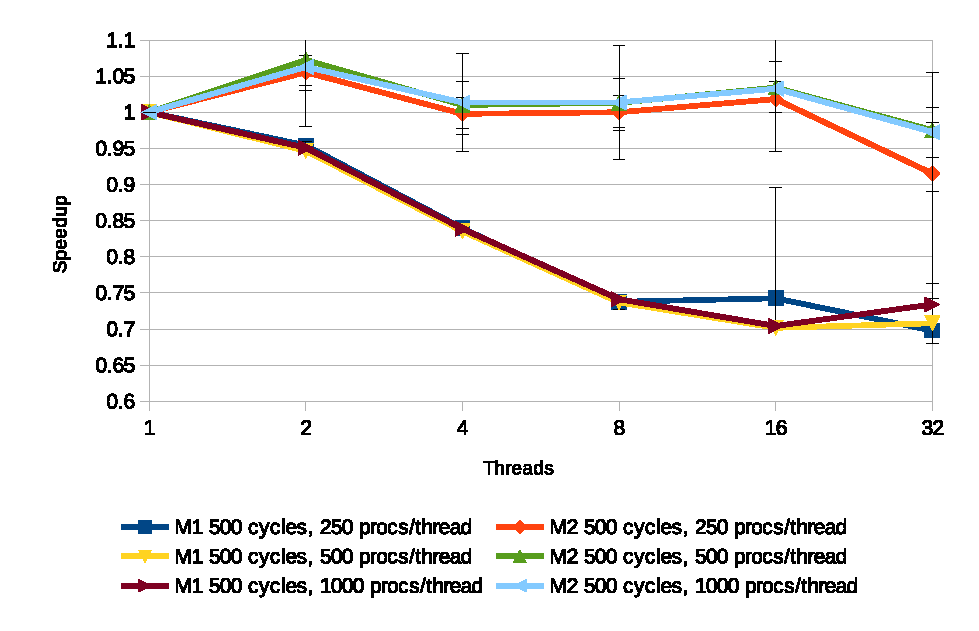
\includegraphics[width=\textwidth]{graphs/weak}
\caption[Weak scaling benchmark]{Weak scaling}
\label{fig:weak}
\end{figure}

\subsection{Discussion}
We can see that the continuous overhead of the atomic variable used in
the worker queue model is still clearly visible and appears to
increase with the level of parallelization. The statically
orchestrated model, on the other hand, produces much better results
and appear to show weak scaling properties with speedups within +/-
0.05. The performance of this model, however appears to drop when
going from 16 to 32 cores. This could be explained by the fact that we
performed the benchmarks on a on a 2x16 core machine This means, that
we cross CPU boundaries when going from 16 to 32 cores.

Contrary to our expectations, the work-per-cycle ratio is not clearly
visible in the results. The explanation for this may simply be that
the work-per-cycle ratios that we used in the benchmark weren't
sufficiently large. In the cycle dominated benchmark we used ratios of
10:1 and 1:10 respectively while in this benchmark we used ratios of
2:1, 1:1 and 1:2.


\section{Uneven workloads}
This benchmark, we attempt to confirm our conjecture that the work
list model will perform better than the statically orchestrated model
for networks coosisting of uneven workloads. This benchmark
essentially repeats the cycle dominated benchmark except that we
divide the processes on the ring evenly into two groups where one
group performs exactly one fourth as much work as the other. This
means, that we use the same process code as \cref{lst:cyclecode}
except that half of the processes will only run for 2500 iterations
instead of 10000 It's important to note that the processes in each of
these groups are laid out sequentially on the ring. since this will force the
statically orchestrated model into its worsts-case distribution of
workload.

The statically orchestrated model will thus spend a lot of time in the
synchronization barrier while the work list model will be able to
distribute load of the network much more evenly across the
threads. This benchmark is indeed very artificial, but it serves the
purpose of showing the strengths of the work list model

\begin{figure}
\centering
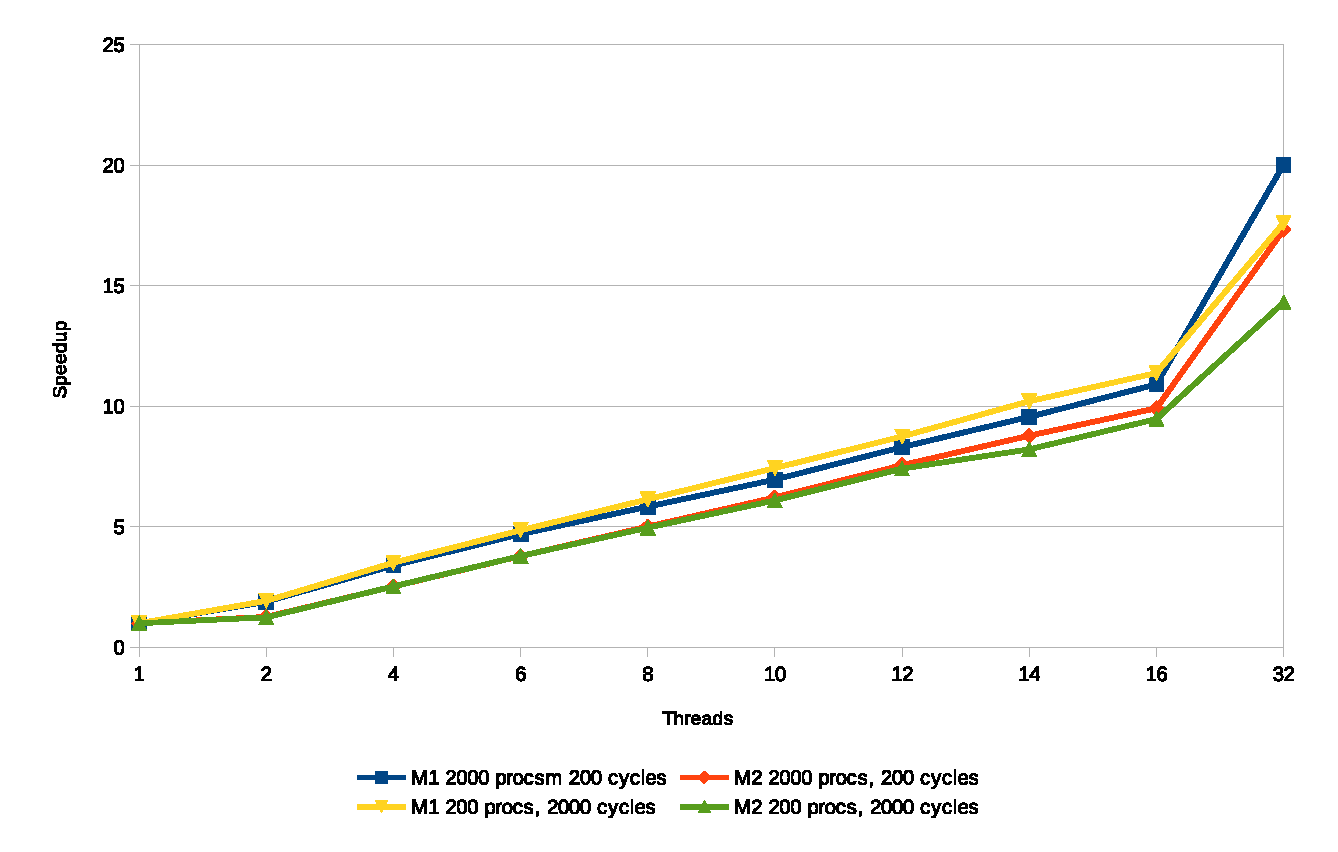
\includegraphics[width=\textwidth]{graphs/uneven}
\caption[Benchmark of uneven workloads]{The performance of the two
  parallelization models when executed on a network consisting of
  processes with a significant workload imbalance}
\label{fig:uneven}
\end{figure}

\subsection{Discussion}
This is the first benchmark where the work list model performed better
than the statically orchestrated model so the fundamental conclusion
is that our conjecture was confirmed. However, the difference between
the two models aren't as significant as we expected. It remains to be
seen whether the work list model would increase its advantage over the
statically orchestrated model if we increased the workload imbalances
between the processes even more but presumably, this would be the
case.

So, once again, the continuous synchronization of the work list model
proves disproportionately expensive.

\section{Future works}

BQueue with work stealing would be nice to implement, but as shown by
relevant benchmark using ``advanved'' datastructures for the process
queue comes at a significant cost. A way to implement work stealing
without increasing the cost of getting a process from the queue is
needed. Linearly pulling processes of a queue has a significant cache
advantage. Using work stealing to pull from ``the reverse'' would
reduce that advantage. 

All benchmarks has been largely artificial since they have been
targeted at exposing the advantages and disadvnatages of the
properties of the execution models that we have proposed  We need more real-world
samples to know where to actually tune the performance of system

More benchmarks:


The results that we have shown, although reasonable, can not be easily
explained by

\subsection{One-shot process orchestration}
In this model, we orchestrate the processes in our network as soon as
possible after execution start and

\subsection{Monte Carlo orchestration}
In this approach, we simply randomize the order of the processes. The
main advantage of this approach is that is computationally cheap
compared to

\subsection{Optimization-based orchestration}
Another way to orchestrate the processes is to use a


\subsection{Adaptive process orchestration}
The benefits of using a oneshot orchestration approach diminishes when
we execute process networks where the processes performs a variable
amount of work per iteration. In these kinds of networks, CPU-core
load distribution will gradually become uneven and suboptimal as the
network execution progresses. In order to keep this from happening and
maximize CPU-core utilization, we need to monitor process execution
time and core idle time as the network execution progresses. This is
what we refer to s adaptive orchestration. This approach, however
introduces another trade-off that we need to consider. producing an

\subsection{Adaptive Monte Carlo process orchestration}

\subsection{Adaptive Optimization-based process orchestration}



%%% Local Variables:
%%% mode: latex
%%% TeX-master: "master"
%%% TeX-command-extra-options: "-enable-write18"
%%% End:
